\section{Computational Complexity Theory}

Computational complexity investigates how many computational resources are required to solve a specific problem. 
We are about to introduce two of the most important classes of problems in classical complexity theory:

\begin{cc}[The Classes \Pt and \NP~{\cite{Arora2006}}]{cc:pnp}

    If we denote \DTIME as the set of decision problems that are solvable in $\mathcal{O}(n^k)$ time by a deterministic Turing Machine, we can define the class \Pt as:

    \[ \mathrm{P} := \bigcup_{k \in \mathbb{N}}(\mathrm{DTIME}(n^k))\]


    \noindent A language $L \subseteq \{0,1\}^*$ is in \NP if there exists a polynomial $p: \mathbb{N} \rightarrow \mathbb{N}$ and a polynomial-time Turing Machine $M$ such that for every $x \in \{0,1\}^*$,

    \[ x \in L \Leftrightarrow \exists u \in \{0,1\}^{p(|x|)} \mathnormal{s.t.~} M(x,u) = 1 \]

    \noindent If $x \in L$ and $u \in \{ 0,1 \}^{p(|x|)}$ satisfy $M(x,u) = 1$, then we call $u$  a \textit{certificate} for $x$.

\end{cc}

\Pt denotes the class of all problems that are \textit{efficiently solvable}, whereas \NP contains all problems whose solution can efficiently be verified. Note that $\Pt \subseteq \NP$, but the opposite is unknown.
\subsection{\NPcn}\label{ch:npc}
A significant discovery in the early 1970s was that some problems in \NP are \textit{at least as hard as} as any other problem in \NP. By spanning a whole ``web of reductions'' \cite{Arora2006} we get strong evidence that none of these problems can be solved efficiently.
The first results in this new field were published independently by Cook \cite{Cook1971} and Levin \cite{Levin1973} after Karp \cite{Karp1972} had introduced the notion of problem reductions.
The Cook-Levin-Theorem \cite{Cook1971} proved that the \SAT (\SATs) problem is \NPc any problem in $NP$ can be reduced to \SATs. 
A single algorithm for one of these problems \NPc problems would instantly give a fast algorithm for the others as well. 
We refer the reader to \cite{Arora2006} for a comprehensive introduction to classical complexity theory.

\begin{definition}[{Reductions, \NP-hardness and \NPcn \cite{Arora2006}}]
We say that a language $A\subseteq \{0,1\}^*$ is \textit{polynomial-time karp reducible} to a language $B \subseteq \{0,1\}^*$ (denote $A \leq_p B$) if there is a poly-time computable function $f: \{0,1\}^* \rightarrow \{0,1\}^*$ such that for every $x \in \{0,1\}^*$, $x \in A$ if and only if $f(x) \in B$.

\noindent We say that a problem $B$ is \NPh if $A \leq_p B$ for every $A \in \NP$ and $B$ is \NPc if additionally $B \in NP$ holds.

\end{definition}
There are thousands of \NPc problems we do not expect to be solvable in polynomial time.
Whether $\Pt \overset{?}{=} \NP$ is still one of the biggest open questions in mathematics and bountied with one million dollars by the \textit{Clay Mathematical Institute} \cite{Fortnow2021}. 
Most of the domination problems like \dom, \sdom, \tdom are \NPc.

% \paragraph{Coping With \NPcn}

We do not expect \NPc problems to have a polynomial-time algorithm, but strategies exist to cope with them. 
We can either give up the exactness of a solution to possibly find fast \textit{approximation algorithms} or abandon the search for a polynomial-time algorithm in favor of finding good \textit{Exact Exponential (EEA) Algorithms} instead.
A third technique is using additional structural parameters of a specific problem instance and therefore \textbf{restricting the input to special cases}. 
This idea led to the development of \textit{parameterized complexity}.

\section{Parameterized Complexity}\label{cha:param}

Introduced by Downey and Fellows \cite{Downey1999a}, parameterized complexity extends the classical theory with a framework that allows a more dimensional analysis of computationally hard problems. 
The idea is to extract an arbitrary parameter $k$ and find an algorithm that is only exponential in a function $f(k)$ but only polynomial in the instance size.
$k$ denotes how complex the problem is: 
$k$ can be seen as a measure of the difficulty of a given instance.
If $k$ is small, the problem can still be considered tractable, although the underlying \NPh problem is generally intractable.
All definitions are taken from \cite{Cygan2015} if not marked otherwise.

\begin{definition}[Parameterized Problem]
    A parameterized problem is a language $L\subseteq\Sigma^*\times \mathbb{N}$ where $\Sigma$ is a finite, fixed alphabet.
    For an instance $(x,k) \in \Sigma^*\times \mathbb{N}$, $k$ is called the \textit{parameter}.

    The \underline{size of an instance} of an instance $(x,k)$ of a parameterized problem is $\abs{(x,k)} = \abs{x} + k$ where the parameter $k$ is encoded in unary by convention.
\end{definition}

\subsection{Fixed-Parameter Tractability}
We say that a problem is \textit{fixed-parameter tractable (fpt)} if problem instances of size $n$ can be solved in $f(k)n^{\mathcal{O}(1)}$ time for some function $f$ independent of $n$. 
Like the class \Pt can be seen as a notion of \textit{tractability} in classical complexity theory, there is an equivalent in parameterized complexity, which we denote as \FPTl (\FPT):

\begin{cc} [The Class \FPT]{cc:fpt}
    A parameterized problem $L\subseteq\Sigma^*\times\mathbb{N}$ is called \textit{fixed-parameter tractable} if there exists an algorithm A (called a \textit{fixed-parameter algorithm}), a computable function $f:\mathbb{N} \rightarrow \mathbb{N}$ and a constant c such that, given $(x,k) \in \Sigma^* \times \mathbb{N}$, the algorithm $\mathcal{A}$ correctly decides whether $(x,k) \in L$ in time bounded by $f(k) \cdot |(x,k)|^c$. The complexity class containing all fixed-parameter tractable problems is called \FPT.
\end{cc}
\subsection{Kernelization}

A kernelization algorithm is a natural and intuitive way to approach problems and is a preprocessing procedure that simplifies parts of an instance before the actual solving algorithm runs. 
The \cref{fig:kernelization} visualizes this idea.
One can introduce different \textit{reduction rules} that iteratively reduce the instance until we are left with a small kernel. 
Ideally, the size of this kernel is merely dependent on the parameter $k$.

\begin{definition}[Kernelization and Reduction Rules]
A \textit{kernelization algorithm} or \textit{kernel} is an algorithm $\mathfrak{A}$ for a parameterized problem $Q$ that given an instance $(I,k)$ of $Q$ runs in polynomial time and returns an equivalent instance $(I', k')$ of $Q$. 
Moreover, we require that $size_{\mathfrak{A}}(k) \leq g(k)$ for some computable function $g:\mathbb{N} \rightarrow \mathbb{N}$.

A \underline{reduction rule} is a function $\phi:\Sigma^* \times \mathbb{N} \rightarrow \Sigma^* \times \mathbb{N}$ that maps an instance $(x,k)$ to an equivalent instance $(x',k')$ such that $\phi$ is computable in time polynomial in $\abs{x}$ and $k$.
A reduction rule is \underline{sound} (or \underline{safe}) if $(I, k) \in Q \Leftrightarrow (I',k') \in Q$.
\end{definition}

We can precisely define the kernel's size after executing a preprocessing algorithm $\mathfrak{A}$.

\begin{definition}[Output Size of a Preprocessing Algorithm] The output size of a preprocessing algorithms $\mathfrak{A}$ is defined as 

    \[\mathrm{size}_{\mathfrak{A}}(k) = \sup\{\abs{I'} + k': (I',k')= \mathfrak{A}(I,k), I \in \Sigma^* \} \]
\end{definition}


$size_{\mathfrak{A}}$ denotes the largest size of any instance $I$ after $\mathfrak{A}$ has been applied.
If no function merely dependent on $k$ can bound it, we consider it to be \emph{infinite}.
If we bound $\mathrm{size}_{\mathfrak{A}}$ by a polynomial in $k$, we say that the problem admits a \textbf{polynomial kernel} or a \textbf{linear} kernel analogously.

\begin{figure}
    \centering
    
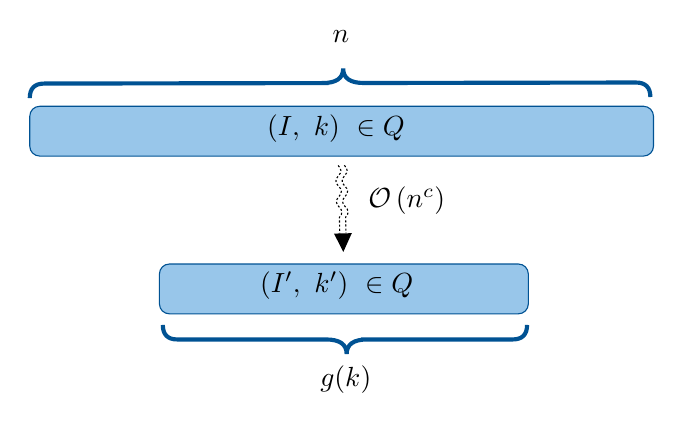
\begin{tikzpicture}[x=0.75pt,y=0.75pt,yscale=-1,xscale=1]
%uncomment if require: \path (0,290); %set diagram left start at 0, and has height of 290
\tikzset{every picture/.style={line width=0.75pt}} %set default line width to 0.75pt        

%Rounded Rect [id:dp2256907851376615] 
\draw  [color={rgb, 255:red, 0; green, 82; blue, 147 }  ,draw opacity=1 ][fill={rgb, 255:red, 152; green, 198; blue, 234 }  ,fill opacity=1 ] (129.8,74.8) .. controls (129.8,72.15) and (131.95,70) .. (134.6,70) -- (425.5,70) .. controls (428.15,70) and (430.3,72.15) .. (430.3,74.8) -- (430.3,89.2) .. controls (430.3,91.85) and (428.15,94) .. (425.5,94) -- (134.6,94) .. controls (131.95,94) and (129.8,91.85) .. (129.8,89.2) -- cycle ;
%Straight Lines [id:da34735862747158275] 
\draw  [dash pattern={on 0.75pt off 0.75pt}]  (281.37,98.46) .. controls (283.08,100.09) and (283.12,101.75) .. (281.49,103.46) .. controls (279.86,105.17) and (279.9,106.83) .. (281.61,108.46) .. controls (283.32,110.09) and (283.36,111.75) .. (281.73,113.46) .. controls (280.1,115.17) and (280.14,116.83) .. (281.85,118.46) .. controls (283.56,120.09) and (283.6,121.75) .. (281.97,123.46) -- (282.08,128.13) -- (282.15,131.13)(278.37,98.54) .. controls (280.08,100.16) and (280.12,101.82) .. (278.49,103.53) .. controls (276.86,105.24) and (276.9,106.9) .. (278.61,108.53) .. controls (280.32,110.16) and (280.36,111.82) .. (278.73,113.53) .. controls (277.1,115.24) and (277.14,116.9) .. (278.85,118.53) .. controls (280.56,120.16) and (280.6,121.82) .. (278.97,123.53) -- (279.08,128.21) -- (279.15,131.21) ;
\draw [shift={(280.87,140.17)}, rotate = 268.63] [fill={rgb, 255:red, 0; green, 0; blue, 0 }  ][line width=0.08]  [draw opacity=0] (8.93,-4.29) -- (0,0) -- (8.93,4.29) -- cycle    ;
%Rounded Rect [id:dp11606859634007116] 
\draw  [color={rgb, 255:red, 0; green, 82; blue, 147 }  ,draw opacity=1 ][fill={rgb, 255:red, 152; green, 198; blue, 234 }  ,fill opacity=1 ] (192.27,150.8) .. controls (192.27,148.15) and (194.42,146) .. (197.07,146) -- (365.2,146) .. controls (367.85,146) and (370,148.15) .. (370,150.8) -- (370,165.2) .. controls (370,167.85) and (367.85,170) .. (365.2,170) -- (197.07,170) .. controls (194.42,170) and (192.27,167.85) .. (192.27,165.2) -- cycle ;
%Shape: Brace [id:dp49500678764931805] 
\draw  [color={rgb, 255:red, 0; green, 82; blue, 147 }  ,draw opacity=1 ][line width=1.5]  (428.8,65.55) .. controls (428.79,60.88) and (426.46,58.55) .. (421.79,58.56) -- (290.81,58.79) .. controls (284.14,58.8) and (280.81,56.48) .. (280.8,51.81) .. controls (280.81,56.48) and (277.48,58.82) .. (270.81,58.83)(273.81,58.82) -- (136.79,59.06) .. controls (132.12,59.07) and (129.79,61.4) .. (129.8,66.07) ;
%Shape: Brace [id:dp39979872340961986] 
\draw  [color={rgb, 255:red, 0; green, 82; blue, 147 }  ,draw opacity=1 ][line width=1.5]  (193.9,175.35) .. controls (193.9,180.02) and (196.23,182.35) .. (200.9,182.35) -- (272.47,182.35) .. controls (279.14,182.35) and (282.47,184.68) .. (282.47,189.35) .. controls (282.47,184.68) and (285.8,182.35) .. (292.47,182.35)(289.47,182.35) -- (362.4,182.35) .. controls (367.07,182.35) and (369.4,180.02) .. (369.4,175.35) ;

% Text Node
\draw (242.9,72.9) node [anchor=north west][inner sep=0.75pt]    {$( I,\ k) \ \in Q$};
% Text Node
\draw (291.67,107.4) node [anchor=north west][inner sep=0.75pt]    {$\mathcal{O}\left( n^{c}\right)$};
% Text Node
\draw (239.5,148.4) node [anchor=north west][inner sep=0.75pt]    {$( I',\ k') \ \in Q$};
% Text Node
\draw (268.5,193.9) node [anchor=north west][inner sep=0.75pt]    {$g( k)$};
% Text Node
\draw (274.5,32.4) node [anchor=north west][inner sep=0.75pt]    {$n$};


\end{tikzpicture}

    \caption[Idea of kernelization]{\textit{The Idea of Kernelization: Reducing an instance $(I,k) \in Q$ of size $n$ to a smaller instance $(I', k') \in Q$ in polynomial time. 
    The resulting size of the kernel is a function $g(k)$ only dependent on $k$.}
    }
    \label{fig:kernelization}
\end{figure}
The following \cref{lemma:fptiskernel} shows the relation between the complexity class \FPT and a kernelization algorithm. 
If we find a kernelization algorithm $\mathfrak{A}$ for a (decidable) problem $P$, we immediately obtain an fpt algorithm.
First, we will run $\mathfrak{A}$ on the given instance in polynomial time and then solve the kernel with an exponential time algorithm.
The total running time is of order $\mathcal{O}(g(f(k)) \cdot \mathrm{poly}(n))$ and hence, fpt.
Surprisingly, also the converse is true:

\begin{lemma}\label{lemma:fptiskernel}
    A parameterized problem $Q$ is \FPT if and only if it admits a kernelization algorithm.
\end{lemma}

 We will use this property in \cref{ch:linkern} to construct a kernel for \psdom and showing membership in \FPT.

\subsection{Reductions and Parameterized Intractability}

It is natural to ask whether all (hard) problems are also fixed-parameter tractable.
The answer is no, and parameterized complexity has another tool to show that a problem is unlikely to be in \FPT.
The idea is to transfer the concepts of \NP-hardness from \Cref{ch:npc} and reductions from the classical setting to the parameterized world.
This raises the need for a new type of reduction that ensures that a reduced instance $(I', k')$ is not only created in fpt time, but the new parameter $k'$ depends only on the size of the parameter in the original instance.

There exists a whole hierarchy of classes $\FPT \subseteq \WONE \subseteq \WTWO \subseteq ... \subseteq \Wt \subseteq ...$, which is known as the \WHIERARCHY.
It is strongly believed that $\FPT \subsetneq \Wt$ and therefore, we do not expect the existence of an algorithm solving any \Wt-hard problem in fpt time.

\begin{definition}[Parameterized Reduction] Let $A,B\subseteq \Sigma^*\times\mathbb{N}$ two parameterized problems. A \textit{parameter preserving reduction} from $A$ to $B$ is an algorithm that, given an instance $(x,k)$ of $A$, outputs an instance $(x', k')$ of $B$ such that:
    \begin{itemize}
        \item $(x,k)$ is a \textcolor{darkgray}{\textbf{yes instance}} of A \textbf{iff} $(x',k')$ is a \textcolor{darkgray}{\textbf{yes instance}} of B,
        \item $k' \leq g(k)$ for some computable function $g$, and
        \item runs in fpt-time $f(k)\cdot |x|^{\mathcal{O}(1)}$ for some computable function f.
    \end{itemize}
\end{definition}

\cref{lem:cfptr,lem:trans} shwon in \cite{Cygan2015} show this definition ensures that reductions are transitive and closed under fpt reductions.

\begin{lemma}[Closed Under fpt-reductions]\label{lem:cfptr}
    If there is a parameterized reduction from $A$ to $B$ and $B \in \FPT$, then $A \in \FPT$.
\end{lemma}

\begin{lemma}[Transitivity] \label{lem:trans}
    If there are parameterized reductions from $A$ to $B$ and from $B$ to $C$, then there is a parameterized reduction from $A$ to $C$.
\end{lemma}

If there exists a parameterized reduction transforming a \Wt-hard problem $A$ to another problem $B$, then $B$ is \Wt-hard as well.
We can define the classes \WONE and \WTWO by giving two problems that are complete for these classes.

\begin{cc}[The Classes \WONE ~{\cite{Downey1995}} and \WTWO ~{\cite{Cygan2015}}]{cc:wi}\begin{align*}
        \\[-2em] & \\[-3em]
        \text{\is is } &\text{\WONE-complete.}\\
        \text{\dom is } &\text{\WTWO-complete.}
    \end{align*}
    A problem $P$ is in the class \WONE (resp. \WTWO) if there is a parameterized reduction from $P$ to \is (\dom).
\end{cc}

A more profound introduction is not required for this work, and we refer the interested reader to \cite{Cygan2015, Fomin2019} for more details.